\documentclass[12pt]{article}
\usepackage{ctex}
\usepackage{amsthm,amsmath,amssymb}
\usepackage{amsfonts}
\usepackage{mathrsfs}
\usepackage{listings}
\usepackage{verbatim}
\usepackage{fancyhdr}
\usepackage{graphicx}
\usepackage{xeCJK}
\usepackage{xcolor}      %代码着色宏包
\usepackage{CJK}         %显示中文宏包
\usepackage{fontspec}
\usepackage{float}
\usepackage{placeins}
\usepackage{subfigure}
\usepackage{bm}
\usepackage[colorlinks,linkcolor=blue]{hyperref}

\lstset{
    basicstyle=\fontspec{Consolas},
    %numbers=left,
    %rulesepcolor=\color{red!20!green!20!blue!20},
    escapeinside=``,
    xleftmargin=2em,xrightmargin=2em, aboveskip=1em,
    %背景框
    framexleftmargin=1.5mm,
    frame=shadowbox,
    %背景色
    backgroundcolor=\color[RGB]{245,245,244},
    %样式
    keywordstyle=\color{blue}\fontspec{Consolas Bold},
    %identifierstyle=\bf,
	breaklines=true,
    numberstyle=\color[RGB]{0,192,192},
    commentstyle=\color[RGB]{96,96,96}\fontspec{Consolas Italic},
    stringstyle=\rmfamily\slshape\color[RGB]{128,0,0},
    %显示空格
    showstringspaces=false
}

\textheight 23cm \textwidth 15cm
\topmargin -1.5cm \oddsidemargin 0.3cm \evensidemargin -0.3cm

\begin{document}
\title {HW1-CAGD}
\date{\today}
\author{阚皓玮}
\maketitle
\section{使用说明}
在matlab中运行Hw1.m脚本文件,出现交互图窗。工具栏中点击红色按钮添加点,蓝色按钮计算结果得到插值图像,绿色按钮清除点和插值图像。

\section{实验内容}
 {\bf Input:} 已知平面内n个点$\overline{P}_j(x_j,y_j),j=1...n$

{\bf Output:} 分别使用多项式函数基及高斯函数基插值拟合这些点的函数f

\section{算法介绍}
给定一组基$B=\{b_1...b_n\}$,我们寻找$B$中基的线性组合,表示拟合函数$f$,使得$f(x_j)=y_j,j=1...n$。i.e.确定$\{\lambda_1,\lambda_2...\lambda_n\}$,令$f(x)=\sum_{j=1}^n\lambda_jb_j(x)$,s.t. $f(x_j)=y_j,j=1...n$。

为了确定$\{\lambda_1...\lambda_n\}$,我们只需计算基函数在数据点$x_j$上的函数值$b_j$,利用待定系数法求解即可得到结果。写成矩阵形式即为:
\begin{equation}
    B=\left(
    \begin{array}{ccc}
            b_1(x_1) & \cdots & b_n(x_1) \\
            \vdots   & \ddots & \vdots   \\
            b_1(x_n) & \cdots & b_n(x_n) \\
        \end{array}
    \right)\ \ \lambda=\left(
    \begin{array}{c}
            \lambda_1 \\
            \vdots    \\
            \lambda_n
        \end{array}
    \right)\ \ Y=\left(
    \begin{array}{c}
            y_1    \\
            \vdots \\
            y_n
        \end{array}
    \right)
\end{equation}
$B\lambda=Y$,通过求解此线性方程即可得到结果。

本次实验中我们使用两组基分别求解,$B^1=\{B^1_i=x^i,i=0...n-1\}$为多项式基,$\displaystyle B^2=\{1,B^2_i(x)=e^{-\frac{(x-x_i)^2}{2\sigma}},i=1...n\}$为高斯基函数,其中$\sigma$缺省为1。

需要注意的是,对于第二组基,需要确定的变量比方程多,我们取基1的系数$\lambda_0$(也就是常数项)为数据点上的函数值$\{y_i,i=1...n\}$的均值进行约束,具体想法将在后面给出。

\section{实验结果}
随着数据点的增加,插值结果图像如下
\begin{figure}[H]
    \subfigure[n=1]{
        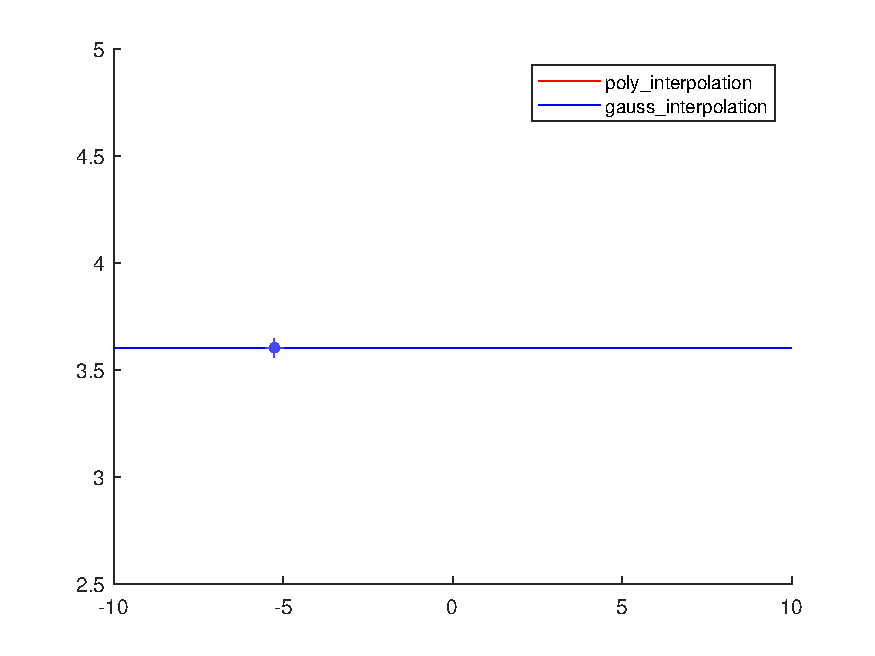
\includegraphics[width=0.43\textwidth]{result/n=1.pdf}
    }
    \subfigure[n=3]{
        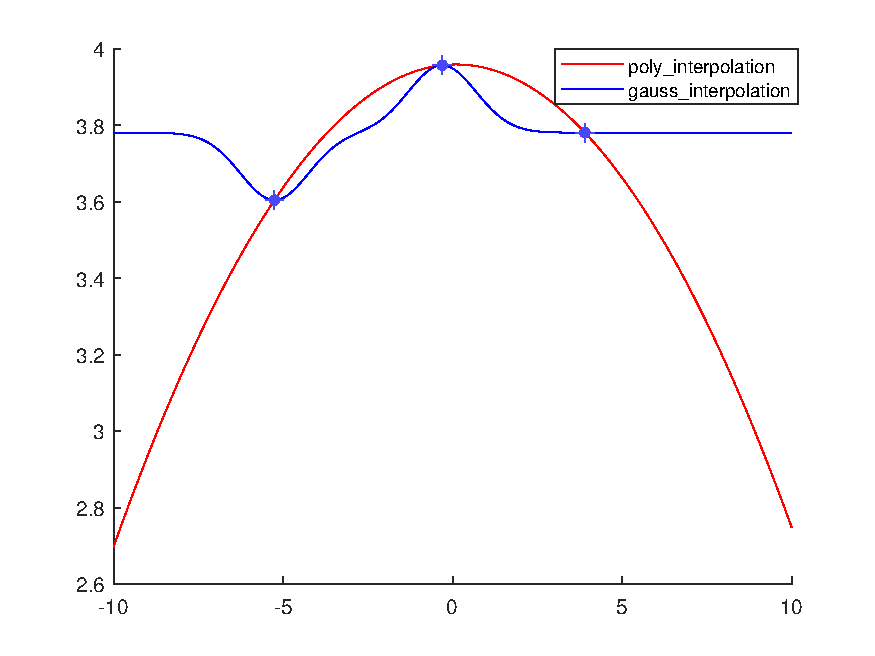
\includegraphics[width=0.43\textwidth]{result/n=3.pdf}
    }
    \subfigure[n=5]{
        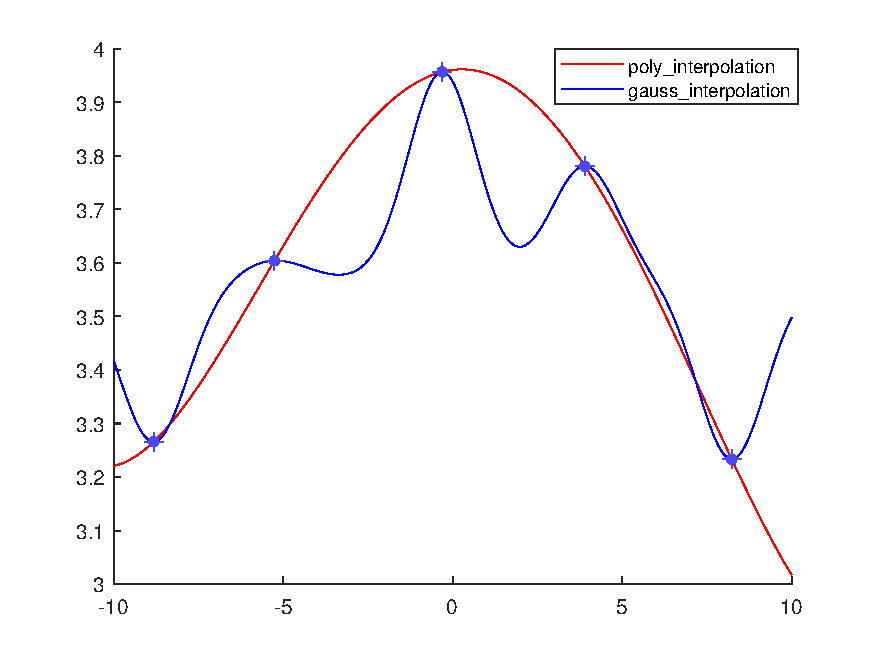
\includegraphics[width=0.43\textwidth]{result/n=5.pdf}
    }
    \subfigure[n=10]{
        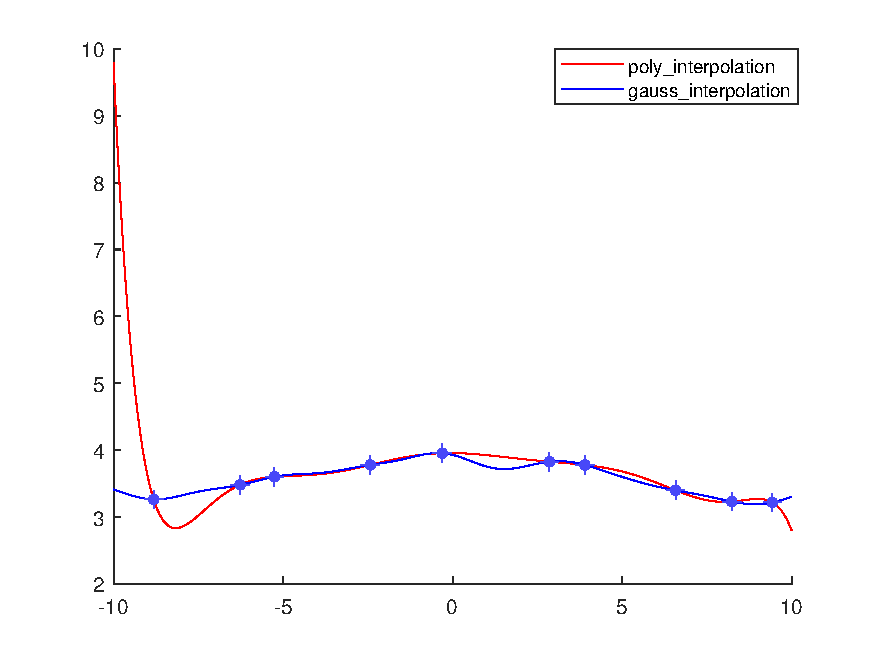
\includegraphics[width=0.43\textwidth]{result/n=10.pdf}
    }
    \subfigure[n=15]{
        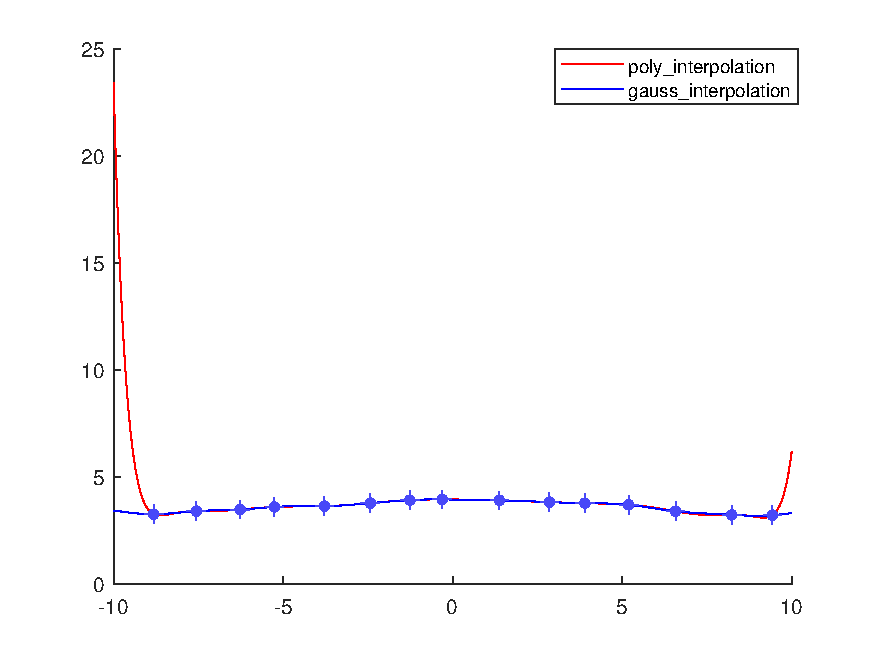
\includegraphics[width=0.43\textwidth]{result/n=15.pdf}
    }
    \quad\quad\quad\
    \subfigure[n=30]{
        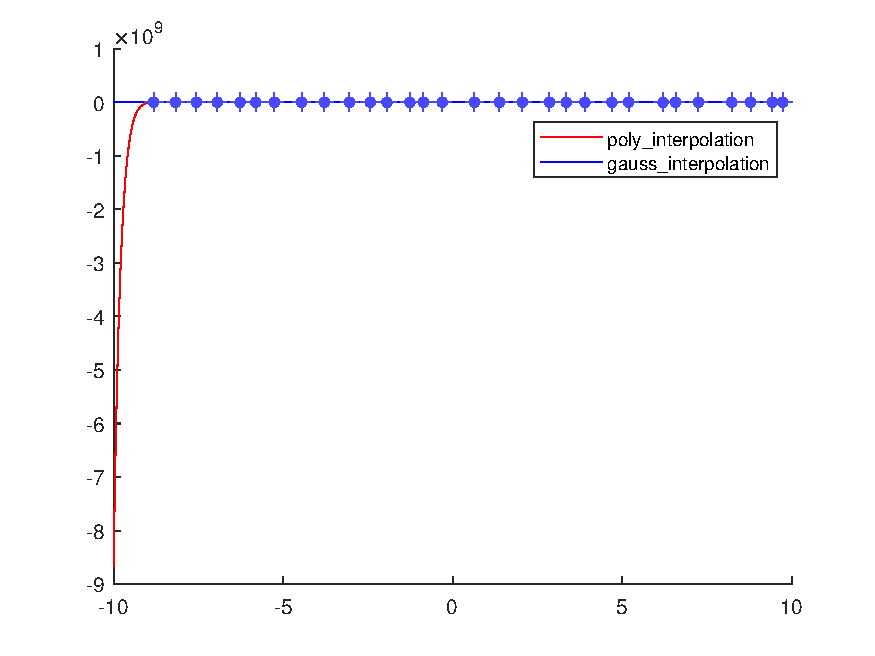
\includegraphics[width=0.43\textwidth]{result/n=30.pdf}
    }

\end{figure}

\section{结果分析及对比}
由结果图可以看出,在插值点数较少时,用多项式插值方法得到的图像较为平稳。而由高斯函数为基得到的函数,由于每一个高斯函数基函数对插值点附近的点影响较大,对远离插值点的点影响较小,每一个插值点在其附近几乎都为一个局部最值,从而会导致一定的震荡。

但随着点的加密,高斯函数作为基函数的拟合趋于平整,但由多项式产生的基函数,由于其多项式的特性,在样本点之外的点的函数值将快速增大(见图(f))。同时,由于多项式为基产生的矩阵为范德蒙矩阵,随着样本点数的增加,得到的系数矩阵的条件数将会增大,导致结果的不准确,在实验中,我们在n=30的时候,条件数的倒数达到了5.774264e-31。由此可见,在样本点数较多时,多项式插值并不是一个好的选择。

\section{高斯函数约束条件的思考}
在高斯函数为基的插值中,我们选择了常数项为各个样本点函数值均值作为约束条件,这是因为每一个高斯函数基对在相应的样本点附近的点影响较大,尤其时当$\sigma$较小时,可能会导致过拟合,加大震荡程度。我们希望减少这种影响,要让样本点尽量分布在常数项两边,方便起见,取常数项为各个样本点函数值的均值。

如果我们将常数项改为低次多项式,同样基于这种考虑,讲样本点划分为多个区间,令多项式在样本点区间内的积分值等于将样本点一一连接得到的函数的积分值,先确定多项式的系数,然后再确定高斯函数基的系数。

\newpage
\appendix
\section{主要算法部分代码}
\lstset{language=MATLAB}
{\bf 多项式插值}
\begin{lstlisting}
function coef = polyInterpolation(points)
%input: coordinates of points
%output: coeficients of poly
[num,~] = size(points);
A = points(:,1).^(0:num-1);
coef = A\points(:,2);
end
\end{lstlisting}

{\bf 高斯函数插值}
\begin{lstlisting}
function coef = gaussInterpolation(points)
%input: coordinates of points
%output: coeficients of gaussian
[num,~]=size(points);
A=repmat(points(:,1),1,num)-repmat(points(:,1)',num,1);
coef = exp(-A.*A/2)\(points(:,2)-mean(points(:,2)));
end
\end{lstlisting}


\end{document}